% Beyond Brown's radial tests -- research note, first-principles draft (2026-10-24).
% Build: pdflatex -> bibtex -> pdflatex x2.  Figures: ../latex/figures/ (make_figures.py, make_figures_v3.py).
% Internal pre-submission checklist lives outside this file (ar/AR-029b packet); nothing here refers to it.
\documentclass[11pt]{amsart}
\usepackage[margin=1in]{geometry}
\usepackage{amsmath,amssymb,amsthm}
\usepackage{graphicx}
\usepackage{booktabs}
\usepackage{array}
\usepackage{enumitem}
\usepackage{microtype}
\usepackage{xcolor}
\definecolor{linkink}{HTML}{1c3f77}
\usepackage[colorlinks=true,linkcolor=linkink,citecolor=linkink,urlcolor=linkink]{hyperref}
\graphicspath{{../latex/figures/}}

\newcommand{\R}{\mathbb{R}}
\newcommand{\dd}{\,\mathrm{d}}
\newcommand{\abs}[1]{\lvert #1\rvert}
\newcommand{\norm}[1]{\lVert #1\rvert}
\newcommand{\fbar}{\bar f}
\DeclareMathOperator{\capa}{cap}
\DeclareMathOperator{\dist}{dist}
\DeclareMathOperator{\Var}{Var}
\DeclareMathOperator{\divg}{div}

\theoremstyle{plain}
\newtheorem{theorem}{Theorem}[section]
\newtheorem{proposition}[theorem]{Proposition}
\newtheorem{lemma}[theorem]{Lemma}
\newtheorem{corollary}[theorem]{Corollary}
\theoremstyle{definition}
\newtheorem{definition}[theorem]{Definition}
\newtheorem{example}[theorem]{Example}
\theoremstyle{remark}
\newtheorem{remark}[theorem]{Remark}

\title[Beyond Brown's radial tests]{Beyond Brown's radial tests:\\ admissibility, parabolicity, and a doubling--Poincar\'e prior that neither test decides}
\author{Oleg Roshka}
\thanks{Independent researcher; ORCID 0009-0009-3075-9417;
\texttt{oleg.roshka@proton.me}.}
\date{24 October 2026}

\begin{document}

\begin{abstract}
For the estimation of a normal mean in $\R^m$ under quadratic loss, Brown (1971)
proved that a generalized Bayes estimator $\delta_F$ is admissible if and only if
a diffusion attached to the marginal $f^*$ of the prior $F$ is recurrent, and
gave two radial tests: a sphere-average test for recurrence and a ray test for
transience. He observed that both tests can be silent. We read his theory as the
potential theory of the weighted Euclidean space $(\R^m,f^*\dd x)$ and ask what
the modern theory of recurrence on weighted manifolds adds inside the zone where
neither test applies. Three results. (A)~If $f^*\dd x$ is doubling and supports a
scale-invariant Poincar\'e inequality, the sphere test is already complete:
recurrence, Brown's sphere test and the ball-volume test are equivalent, so
geometric criteria can add decidable cases only on the inadmissible side.
(B)~They do add one. An explicit prior on $\R^3$, supported near a lattice of
circles at dyadic scales with spacing equal to the square root of the scale, is
doubling and Poincar\'e, silences both of Brown's tests, and is transient by the
ball-volume test; its generalized Bayes estimator is inadmissible. (C)~Outside
the doubling--Poincar\'e class the zone is two-sided: the same circles placed on
one surface per scale give an admissible estimator, decided by a flux bound along
a non-spherical exhaustion, and a logarithmic product prior gives an inadmissible
one, decided by product heat kernels. A comparison lemma shows that any positive
weight with Lipschitz logarithm is, up to constants, the marginal of a prior, so
that explicit weights may be used throughout.
\end{abstract}

\maketitle
% Running heads: the short title on every page; the author is named once, on the first page.
\markboth{Beyond Brown's radial tests}{Beyond Brown's radial tests}

\section{Introduction}\label{sec:intro}

Let $X\sim N_m(\theta,I_m)$ and consider estimators of $\theta$ under quadratic
loss. For a $\sigma$-finite measure $F$ on $\R^m$ with finite Gaussian marginal
$f^*=\varphi*F$, where $\varphi$ is the standard normal density, the generalized
Bayes estimator is
\[
\delta_F(x)=x+\nabla\log f^*(x) .
\]
Brown \cite{brown1971} showed that every admissible estimator is of this form
and characterized admissibility by the behaviour of a diffusion: let
$\{Z_t\}$ be the diffusion on $\R^m$ with generator
$\Delta+\nabla\log f^*\cdot\nabla$, the weighted Laplacian of the measure
$\mu=f^*\dd x$. Then $\delta_F$ is inadmissible if $\{Z_t\}$ is transient, and
admissible if $\{Z_t\}$ is recurrent and the drift $\nabla\log f^*$ is bounded.
Since the recurrence of $\{Z_t\}$ is the \emph{parabolicity} of the weighted
Euclidean space $W_F=(\R^m,\delta_{ij},f^*\dd x)$, Brown's theorem places the
admissibility problem inside the potential theory of weighted manifolds, a
subject that has developed independently since
\cite{lyonssullivan1984,grigoryan1985,grigoryan1999}. The statistical
literature has long used the Dirichlet-form formulation of Brown's criterion
\cite{johnstonelalley1984,johnstone1986,eaton1992,takanashi2023}; the geometric
reading, and the tests it brings, are the subject of this note.

Brown gave two tests that depend only on radial information. Write
$\fbar(r)$ for the mean of $f^*$ over the sphere $\{\abs x=r\}$. His sphere
test says that $\int_1^\infty\dd r/(r^{m-1}\fbar(r))=\infty$ implies
recurrence; his ray test says that if the ray integrals
$\int_1^\infty\dd r/(r^{m-1}f^*(r\varphi))$ are uniformly bounded on a set of
directions $\varphi$ of positive measure, then $\delta_F$ is inadmissible. He
remarked \cite[p.~900]{brown1971} that there are marginals on which neither test
applies. We call this set of marginals \emph{Brown's undecided zone}.

The geometric literature knows the sphere test as the sphere-area parabolicity
test \cite[Thm.~7.5]{grigoryan1999}, and knows further tests with no
statistical counterpart: the ball-volume test of Karp, Varopoulos and
Grigor'yan, which is an equivalence when the measure is doubling and supports a
Poincar\'e inequality \cite[Thm.~11.1]{grigoryan1999}, and the flux test along
an arbitrary exhaustion \cite[Thm.~7.6]{grigoryan1999}. Our question is what
these add inside Brown's undecided zone. The answer has three parts.

\begin{itemize}[leftmargin=2em,itemsep=3pt]
\item[(A)] \emph{Inside the doubling--Poincar\'e class, Brown's sphere test is
complete} (Theorem~\ref{thm:A}). If $f^*\dd x$ is doubling and supports a
scale-invariant Poincar\'e inequality, then recurrence, the divergence of the
sphere integral, and the divergence of the volume integral
$\int^\infty r\dd r/\mu(B_r)$ are equivalent. So for such priors with bounded
drift, $\delta_F$ is admissible if and only if Brown's 1971 test says so, and
geometric criteria can only decide cases on the inadmissible side.
\item[(B)] \emph{They do decide one} (Theorem~\ref{thm:B}). We construct a prior
on $\R^3$ whose marginal is doubling and Poincar\'e, on which both of Brown's
tests are silent (every ray integral diverges, the sphere integral converges),
and whose volume grows like $r^3$; the ball-volume test shows transience and
$\delta_F$ is inadmissible. The construction places circles of radius
$\asymp2^k$ in the shell $2^k\le\abs x<2^{k+1}$ at mutual distance $\asymp
2^{k/2}$, so that their angular positions cover every direction while no
coherent surface of small weight forms.
\item[(C)] \emph{The zone is two-sided} (Section~\ref{sec:zone}). Placing the
same circles on one surface per shell produces a prior on which both tests are
silent and which is nevertheless recurrent, hence admissible; the proof is a
flux bound along the surfaces. A logarithmic product prior is transient, hence
inadmissible, by product heat kernels. Neither prior is doubling and Poincar\'e,
and Theorem~\ref{thm:A} says why the first cannot be.
\end{itemize}

A comparison lemma (Lemma~\ref{lem:lip}) shows that any positive weight $w$
with Lipschitz logarithm satisfies $c\,w\le\varphi*w\le C\,w$ with bounded
drift, so that every explicit weight below is, up to constants, the marginal of
the prior $F=w\dd\theta$. All statements about recurrence, doubling, Poincar\'e
inequalities and Brown's tests are stable under such comparability.

The examples of Section~\ref{sec:zone} connect to the question of Johnstone and
Lalley \cite{johnstonelalley1984}, whether any generalized Bayes estimator that
is not proper Bayes is immune to the Stein effect under products; their theory
decides the product example and our construction in Theorem~\ref{thm:B} is the
non-product counterpart. The same dichotomy between parabolic and non-parabolic
geometry governs Komaki's theory of shrinkage priors for predictive densities,
where a prior asymptotically dominating the Jeffreys prior exists if and only if
the Fisher manifold of the model is non-parabolic \cite{komaki2006};
Appendix~\ref{app:komaki} records that parallel and the identity that expresses
Komaki's risk reduction through Perelman's weighted scalar curvature.
% TODO (pre-submission): compare with Brown & Hwang (1982), "A unified
% admissibility proof", the standard non-radial sufficient condition, and state
% whether the lattice prior of Theorem B is covered by it.

\paragraph{Organization.} Section~\ref{sec:prelim} fixes notation, restates
Brown's theorems in geometric language, proves the comparison lemma, and records
the volume criterion. Section~\ref{sec:reach} proves Theorem~\ref{thm:A} and
locates the undecided zone through the spherical $A_2$ ratio.
Section~\ref{sec:lattice} constructs the prior of Theorem~\ref{thm:B} and proves
its properties. Section~\ref{sec:zone} gives the two further examples.
Section~\ref{sec:numerics} reports numerical companions to the proofs, and
Section~\ref{sec:discussion} discusses what the geometric criteria add and what
remains open.

\section{Preliminaries}\label{sec:prelim}

\subsection{Notation}
Throughout, $m\ge2$, $B(x,\rho)$ is the open Euclidean ball, $B_r=B(0,r)$, and
$\omega_{m-1}$ the area of the unit sphere. For a positive locally integrable
weight $w$ on $\R^m$ we write $\mu=w\dd x$ and $V(r)=\mu(B_r)$. For $r\ge1$ let
$\fbar(r)$ and $A(r)$ be the means of $w$ and of $1/w$ over the sphere
$\{\abs x=r\}$, and $Q(r)=\fbar(r)A(r)\ge1$ (Jensen) the \emph{spherical $A_2$
ratio}. The measure $\mu$ is \emph{doubling} if $\mu(B(x,2\rho))\le
D\,\mu(B(x,\rho))$ for all balls, and supports the \emph{scale-invariant
Poincar\'e inequality} if
\begin{equation}\label{eq:poincare}
\int_B\abs{u-u_B}^2\dd\mu\ \le\ C_P\,\rho^2\int_B\abs{\nabla u}^2\dd\mu
\qquad\text{for every ball $B$ of radius $\rho$ and every $u\in C^1(\bar B)$},
\end{equation}
where $u_B$ is the $\mu$-mean of $u$ on $B$. We say that $\mu$ (or $w$) is
\emph{D+P} if both hold. The best constant in \eqref{eq:poincare} on a given
ball is $1/(\lambda_1(B)\rho^2)$, where $\lambda_1(B)$ is the first nonzero
Neumann eigenvalue of the weighted Laplacian $-w^{-1}\divg(w\nabla\cdot)$ on
$B$; this is how the inequality is tested numerically in
Section~\ref{sec:numerics}.

The weighted space $(\R^m,\delta_{ij},\mu)$ carries the Dirichlet form
$\mathcal E(u)=\int\abs{\nabla u}^2\dd\mu$ and the weighted Brownian motion with
generator $\Delta+\nabla\log w\cdot\nabla$. It is \emph{parabolic} if the
capacity of some (equivalently every) ball vanishes,
$\capa(B_1)=\inf\{\mathcal E(j):j\in C_c^\infty,\ j\ge1\text{ on }B_1\}=0$,
equivalently if the weighted Brownian motion is recurrent
\cite[Thm.~5.1]{grigoryan1999}; otherwise it is \emph{non-parabolic} or
\emph{transient}.

\subsection{Brown's theorems}
We restate the results of \cite{brown1971} that we use, in the notation above
with $w=f^*$.

\begin{theorem}[Brown \cite{brown1971}]\label{thm:brown}
Let $F$ be a $\sigma$-finite measure on $\R^m$ with $f^*=\varphi*F<\infty$, and
let $\{Z_t\}$ be the weighted Brownian motion of $(\R^m,f^*\dd x)$.
\begin{enumerate}[label=\textup{(\alph*)},leftmargin=2em,itemsep=2pt]
\item \textup{(Thm.~4.3.1)} $\{Z_t\}$ is transient if and only if
$\capa(B_1)>0$ in $(\R^m,f^*\dd x)$.
\item \textup{(Thm.~5.1.1)} If $\{Z_t\}$ is transient, $\delta_F$ is
inadmissible. If $\{Z_t\}$ is recurrent and $\sup\abs{\nabla\log f^*}<\infty$,
$\delta_F$ is admissible.
\item \textup{(Thm.~6.3.1)} If $F$ is spherically symmetric, $\delta_F$ is
inadmissible if and only if
\[
\int_1^\infty\frac{\dd r}{r^{m-1}f^*(r)}<\infty .
\]
\item \textup{(Thm.~6.4.3, sphere test)} If
\[
\int_1^\infty\frac{\dd r}{r^{m-1}\fbar(r)}=\infty ,
\]
then $\{Z_t\}$ is recurrent; hence $\delta_F$ is admissible if moreover
$\nabla\log f^*$ is bounded.
\item \textup{(Thm.~6.4.4, ray test)} If a set $\Omega$ of directions of
positive surface measure satisfies
\[
\sup_{\varphi\in\Omega}\int_1^\infty\frac{\dd r}{r^{m-1}f^*(r\varphi)}<\infty ,
\]
then $\delta_F$ is inadmissible.
\end{enumerate}
\end{theorem}

Brown's proofs are those of the corresponding geometric statements: (a) is the
Dirichlet principle for the capacity of $B_1$; (d) uses the radial test
functions $j_i(x)=c_i\int_{\abs x}^{i}\dd r/(r^{m-1}\fbar(r))$, whose energy
tends to zero, exactly as in the sphere-area test of
\cite[Thm.~7.5]{grigoryan1999}; (e) integrates a one-dimensional capacity
bound along rays. We say that the sphere test is \emph{silent} on $F$ when its
integral converges, and that the ray test is silent when no set of directions
of positive measure has uniformly bounded ray integrals. Brown's undecided zone
is the set of $F$ on which both are silent. Table~\ref{tab:dict} collects the
dictionary.

\begin{table}[t]
\caption{Brown's admissibility theory read as potential theory of
$W_F=(\R^m,\delta,f^*\dd x)$. Theorem numbers refer to \cite{brown1971} and
\cite{grigoryan1999}.}
\label{tab:dict}
\small
\begin{tabular}{@{}>{\raggedright\arraybackslash}p{0.44\textwidth}>{\raggedright\arraybackslash}p{0.50\textwidth}@{}}
\toprule
statistics & weighted potential theory \\
\midrule
generalized Bayes estimator $\delta_F=x+\nabla\log f^*$ & weighted space $W_F$ with measure $f^*\dd x$ \\
Brown's diffusion $\{Z_t\}$ & weighted Brownian motion, generator $\Delta+\nabla\log f^*\cdot\nabla$ \\
Brown's energy infimum (Thm.~4.3.1) & capacity of the unit ball (Grigor'yan, Thm.~5.1) \\
$\delta_F$ admissible, bounded drift (Thm.~5.1.1) & $W_F$ parabolic \\
spherical $F$ (Thm.~6.3.1) & model-manifold test $\int^\infty\dd r/S(r)$, $S(r)=\omega_{m-1}r^{m-1}f^*(r)$ \\
sphere test (Thm.~6.4.3) & sphere-area parabolicity test (Grigor'yan, Thm.~7.5) \\
--- & ball-volume test $\int^\infty r\dd r/V(r)=\infty$ (Thm.~7.3); an equivalence under D+P (Thm.~11.1) \\
--- & flux test along an arbitrary exhaustion (Thm.~7.6); Lemma~\ref{lem:thomson} below \\
MLE admissible iff $m\le2$ (Stein \cite{stein1956}) & Brownian motion recurrent iff $m\le2$ \\
\bottomrule
\end{tabular}
\end{table}

\begin{remark}[priority]\label{rem:priority}
Grigor'yan \cite[p.~178]{grigoryan1999} attributes the sphere-area test for
Riemannian manifolds to Lyons--Sullivan \cite{lyonssullivan1984} and to
\cite{grigoryan1985}. Brown's Theorem~6.4.3 is the same test on $W_F$, with the
same proof, thirteen years earlier, and his Theorem~4.3.1 is the capacity
characterization of parabolicity. In the sources we have read, neither
literature cites the other.
\end{remark}

\subsection{Explicit weights are marginals}
Brown's theorems concern Gaussian marginals $f^*=\varphi*F$. The weights we
construct are explicit functions of the distance to a set, which are not
Gaussian marginals as they stand. The following lemma removes the distinction.

\begin{lemma}[comparison]\label{lem:lip}
Let $w>0$ on $\R^m$ be locally integrable with $\log w$ Lipschitz with constant
$L$, and let $f^*=\varphi*w$, the marginal of the prior $F=w\dd\theta$. Then
\begin{enumerate}[label=\textup{(\roman*)},leftmargin=2em,itemsep=1pt]
\item $c_L\,w\le f^*\le C_L\,w$ with $c_L=E\,e^{-L\abs Z}>0$ and
$C_L=E\,e^{L\abs Z}<\infty$, $Z\sim N(0,I_m)$;
\item $\abs{\nabla\log f^*}\le L$;
\item $F$ is $\sigma$-finite and $f^*<\infty$, so Theorem~\ref{thm:brown}
applies to $\delta_F$;
\item the spaces $(\R^m,w\dd x)$ and $(\R^m,f^*\dd x)$ have comparable Dirichlet
forms, hence the same parabolicity type; doubling constants, Poincar\'e
constants, sphere means, ray integrals and ball volumes of the two weights are
comparable, so Brown's tests are silent for $w$ if and only if they are silent
for $f^*$, and $w$ is D+P if and only if $f^*$ is.
\end{enumerate}
\end{lemma}

\begin{proof}
From $e^{-L\abs z}\le w(x+z)/w(x)\le e^{L\abs z}$, integration against
$\varphi$ gives (i); $\nabla f^*=\varphi*(w\nabla\log w)$ and
$\abs{\nabla\log w}\le L$ give (ii); (iii) is immediate, and (iv) follows from
(i) applied to $\int\abs{\nabla u}^2w\dd x$ and to the integrals that define the
other quantities, together with Theorem~\ref{thm:brown}(a).
\end{proof}

For $m=3$ and $L=2$ one has $C_L=73.8$ and $c_L=0.085$. Some of the weights
below are marginals exactly: for $y,Z\in\R^2$,
$E\abs{y+Z}^4=\abs y^4+8\abs y^2+8$, so the weight $(1+\abs y^2)^2$ is, up to
constants, the marginal of $\dist(\theta,\ell)^4\dd\theta$ for a line
$\ell\subset\R^3$.

\subsection{The volume criterion under doubling and Poincar\'e}
The following is the theorem of the geometric literature on which
Theorem~\ref{thm:A} rests.

\begin{theorem}[Grigor'yan; Saloff-Coste; Sturm]\label{thm:volume}
Let $w$ be D+P on $\R^m$. Then $(\R^m,w\dd x)$ is parabolic if and only if
\begin{equation}\label{eq:volume}
\int_1^\infty\frac{r\dd r}{V(r)}=\infty .
\end{equation}
\end{theorem}

\begin{proof}[Sources]
By Lemma~\ref{lem:lip} we may take $w$ smooth, so that $-w^{-1}\divg(w\nabla\cdot)$
is a uniformly elliptic operator with smooth coefficients, symmetric with
respect to $\mu$. For such operators Saloff-Coste proved that doubling together
with the Poincar\'e inequality is equivalent to the parabolic Harnack inequality
\cite[Thm.~3.1]{saloffcoste1992} and implies two-sided Gaussian bounds for the
heat kernel \cite[Thm.~4.2]{saloffcoste1992}; see also \cite{grigoryan1991}
and, for local Dirichlet spaces, \cite{sturm1996}. In particular the upper bound
$p(t,x,x)\le C/V(x,\sqrt t)$ holds, which together with doubling is equivalent to the
relative Faber--Krahn inequality \cite[remark after Thm.~11.1]{grigoryan1999}.
Under the relative Faber--Krahn inequality, non-parabolicity is equivalent to
the convergence of the integral in \eqref{eq:volume}
\cite[Thm.~11.1]{grigoryan1999}; the weighted-manifold form of these arguments is
in \cite{grigoryan2009}. The implication ``\eqref{eq:volume} $\Rightarrow$
parabolic'' holds without any hypothesis \cite[Thm.~7.3]{grigoryan1999}.
\end{proof}

\begin{corollary}[the sphere test dominates the volume test]\label{cor:cs}
For any positive weight, divergence of $\int^\infty r\dd r/V(r)$ implies
divergence of $\int^\infty\dd r/(r^{m-1}\fbar(r))$.
\end{corollary}

\begin{proof}
$V'(r)=\omega_{m-1}r^{m-1}\fbar(r)$. By the Cauchy--Schwarz inequality on
$[R,2R]$, $R^2=\bigl(\int_R^{2R}\dd r\bigr)^2\le\int_R^{2R}V'\dd r\cdot
\int_R^{2R}\dd r/V'\le V(2R)\int_R^{2R}\dd r/V'$, while
$\int_R^{2R}r\dd r/V\le2R^2/V(R)$. Summing over $R=2^j$, divergence of the
volume integral forces $\sum_j4^j/V(2^{j+1})=\infty$ and hence divergence of
$\int\dd r/V'$.
\end{proof}

\section{The reach of the radial tests}\label{sec:reach}

\begin{theorem}[the sphere test is complete under D+P]\label{thm:A}
Let $w$ be D+P on $\R^m$, $m\ge2$. Then the following are equivalent:
\begin{enumerate}[label=\textup{(\roman*)},leftmargin=2em,itemsep=1pt]
\item $(\R^m,w\dd x)$ is parabolic;
\item $\int_1^\infty\dd r/(r^{m-1}\fbar(r))=\infty$ (Brown's sphere test fires);
\item $\int_1^\infty r\dd r/V(r)=\infty$ (the ball-volume test fires).
\end{enumerate}
Consequently, if $f^*$ is D+P with bounded drift, $\delta_F$ is admissible if
and only if Brown's sphere test fires. The ray test implies transience but is
not necessary for it: the weight of Theorem~\ref{thm:B} is D+P and transient
with the ray test silent.
\end{theorem}

\begin{proof}
(iii)$\Leftrightarrow$(i) is Theorem~\ref{thm:volume}. (ii)$\Rightarrow$(i) is
Brown's sphere test, Theorem~\ref{thm:brown}(d). (i)$\Rightarrow$(iii) is
Theorem~\ref{thm:volume} again, and (iii)$\Rightarrow$(ii) is
Corollary~\ref{cor:cs}. The statement about $\delta_F$ is
Theorem~\ref{thm:brown}(b) with Lemma~\ref{lem:lip} if $f^*$ is only
comparable to a D+P weight. The last sentence is Theorem~\ref{thm:B}.
\end{proof}

Thus, within the D+P class, the geometric literature adds nothing on the
admissible side, where Brown's 1971 sphere test is necessary and sufficient, and
it can add exactly one kind of case on the inadmissible side: a transient weight
along whose every ray the escape to infinity is expensive. Theorem~\ref{thm:B}
shows that this case occurs. The next two lemmas locate the undecided zone more
precisely and explain why one spatial dimension is not enough to enter it.

\begin{lemma}[bounded spherical $A_2$ ratio]\label{lem:a2}
Suppose $\sup_{r\ge1}Q(r)=C<\infty$. If
$\int_1^\infty\dd r/(r^{m-1}\fbar(r))=\infty$ then $(\R^m,w\dd x)$ is parabolic;
if the integral converges then the ray test fires. Hence Brown's two tests are
exhaustive on weights with bounded spherical $A_2$ ratio, and every weight in
the undecided zone has $Q(r)\to\infty$ along a sequence.
\end{lemma}

\begin{proof}
The first case is Theorem~\ref{thm:brown}(d). In the second, let
$R(\varphi)=\int_1^\infty\dd r/(r^{m-1}w(r\varphi))$. By Fubini its mean over
the unit sphere is $\int_1^\infty A(r)\dd r/r^{m-1}\le
C\int_1^\infty\dd r/(r^{m-1}\fbar(r))<\infty$, so by Chebyshev's inequality the
set $\{\varphi:R(\varphi)\le2\,\mathrm{mean}\,R\}$ has at least half the surface
measure, and $R$ is bounded on it: the hypothesis of
Theorem~\ref{thm:brown}(e).
\end{proof}

\begin{lemma}[one-dimensional D+P forces $A_2$]\label{lem:1d}
Let $v>0$ be continuous on $\R$ with $\mu_1=v\dd t$ doubling, $\mu_1(2I)\le
D\mu_1(I)$ for all intervals $I$, and satisfying
$\int_I\abs{u-u_I}^2\dd\mu_1\le C\abs I^2\int_I\abs{u'}^2\dd\mu_1$ for all
intervals. Then, with $\nu_1=v^{-1}\dd t$,
$\mu_1([-r,r])\,\nu_1([-r,r])\le32\,CD^3r^2$ for every $r>0$. Consequently the
product weight $w(x)=v(x_1)$ on $\R^m$, $m\ge3$, has bounded spherical $A_2$
ratio, and $\delta_F$ is inadmissible for every such prior.
\end{lemma}

\begin{proof}
Take $I=[-2r,2r]$ and the test function $u=0$ on $[-2r,-r]$, $u=1$ on $[r,2r]$,
and $u(t)=\nu_1([-r,t])/\nu_1([-r,r])$ in between, which minimizes the energy
across the middle segment: $\int_I\abs{u'}^2\dd\mu_1=1/\nu_1([-r,r])$. A function
equal to $0$ on a set of measure $a$ and to $1$ on a set of measure $b$ has
weighted variance at least $ab/(a+b)\ge\frac12\min(a,b)$. Since $[-r,r]$ is
contained in the eightfold dilates of $[r,2r]$ and of $[-2r,-r]$, doubling gives
$\mu_1([r,2r])\ge\mu_1([-r,r])/D^3$ and likewise on the left, and the Poincar\'e
inequality reads $\mu_1([-r,r])/(2D^3)\le C(4r)^2/\nu_1([-r,r])$. For the product
weight, the sphere means are weighted means of $v$ and $1/v$ over $[-r,r]$
with a kernel bounded above and bounded below on $[-r/\sqrt2,r/\sqrt2]$, so by
doubling $\fbar(r)\asymp\mu_1([-r,r])/r$ and $A(r)\lesssim\nu_1([-r,r])/r$,
whence $Q$ is bounded. Doubling also gives reverse doubling,
$\mu_1([-r,r])\ge cr^\varepsilon$, so $\int^\infty\dd r/(r^{m-1}\fbar)\lesssim
\int^\infty r^{2-m-\varepsilon}\dd r<\infty$ for $m\ge3$, and Lemma~\ref{lem:a2}
gives inadmissibility.
\end{proof}

Both hypotheses are needed: $v(t)=(1+\abs t)^2$ is doubling but fails the
Poincar\'e inequality, because the valley at $0$ is a bottleneck between two
heavy sides, and $v(t)=(1+\abs t)^{-2}$ satisfies the Poincar\'e inequality
but is not doubling; in both cases $\mu_1\nu_1/r^2$ grows like $r$
(Figure~\ref{fig:oned}b,c). The mechanism of Lemma~\ref{lem:1d} is that a valley
in one dimension has co-dimension one and disconnects the interval. In $\R^m$,
$m\ge3$, a valley along a curve has co-dimension two, does not disconnect, and
the lemma fails:

\begin{theorem}[co-dimension-two valleys]\label{thm:cyl}
For $m\ge3$ and $\alpha\ge0$ the weight
$w(x)=(1+x_1^2+\dots+x_{m-1}^2)^{\alpha/2}$ on $\R^m$, a power of the distance to
the $x_m$-axis, is D+P. For $\alpha>m-1$ its spherical $A_2$ ratio satisfies
$Q(r)\asymp r^{\alpha-(m-1)}\to\infty$.
\end{theorem}

\begin{proof}
Bj\"orn \cite[Prop.~6]{bjorn2001}, generalizing Chanillo and Wheeden, proves
that for $x=(x',x'')$ with $x'\in\R^k$, $2\le k\le n$, any $v\in A_p$, points
$a_j\in\R^k$ and exponents $\gamma_0,\gamma_j\ge0$, the weight
$v(x)(1+\abs{x'})^{\gamma_0}\prod_j\bigl(\abs{x'-a_j}/(1+\abs{x'-a_j})\bigr)^{\gamma_j}$
on $\R^n$ is $p$-admissible, that is, doubling and supporting the weak
$(1,p)$-Poincar\'e inequality. Take $n=m$, $k=m-1$, $v\equiv1$,
$\gamma_0=\alpha$, no $a_j$, and $p=2$; since $(1+\abs{x'})^\alpha\asymp
(1+\abs{x'}^2)^{\alpha/2}$, the weight is doubling and supports the weak
$(1,2)$-Poincar\'e inequality in the sense of \cite[(5), p.~7]{hajlaszkoskela2000},
which under doubling self-improves to the strong $(2,2)$ form
\eqref{eq:poincare}: \cite[Thm.~5.1]{hajlaszkoskela2000} raises the exponent
on the left to any $h<sp/(s-p)$, with the energy on a dilated ball, and
\cite[Thm.~9.7]{hajlaszkoskela2000} removes the dilation on any weak John
domain, in particular on a ball (the exponent $s$ in the lower mass bound
exists for every doubling measure, \cite[Lemma~14.6]{hajlaszkoskela2000}). For the
asymptotics parameterize the sphere $\{\abs x=r\}$ by $\abs{x'}=r\sin\theta$;
then $\fbar(r)\asymp r^\alpha$, and for $\alpha>m-1$ the integral of $1/w$
concentrates on the polar caps $\theta\lesssim1/r$, giving
$A(r)\asymp r^{-(m-1)}$.
\end{proof}

So Lemma~\ref{lem:1d} is a one-dimensional statement, and weights in the
undecided zone that are D+P must have valleys of co-dimension at least two. The
ray test, however, is silent only if \emph{every} direction (up to a null set)
meets cheap regions at infinitely many scales, which a single line does not
achieve. The construction of the next section makes the valleys sweep every
direction without ever forming a surface.

\section{A doubling--Poincar\'e prior that neither test decides}\label{sec:lattice}

\subsection{The construction}\label{sec:construction}
Work in $\R^3$ with spherical coordinates $(r,\theta,\phi)$, $\theta\in[0,\pi]$
the polar angle. For $k\ge4$ put
\[
N_k=2^{k+2},\qquad L_k=2^{\lceil k/2\rceil},\qquad M_k=N_k/L_k,\qquad
s_k=2^{k/2}.
\]
Shell $k$ is $\{2^k\le\abs x<2^{k+1}\}$. For $0\le i<L_k$ and $0\le j<M_k$ let
$n=jL_k+i$ and let $\Gamma_{k,i,j}$ be the latitude circle
\[
\Gamma_{k,i,j}=\Bigl\{\abs x=2^k+i\,\frac{2^k}{L_k},\ \ \theta=\theta_n:=
\frac{\pi(n+\tfrac12)}{N_k}\Bigr\}.
\]
Since $(i,j)\mapsto n$ is a bijection onto $\{0,\dots,N_k-1\}$, the $N_k$
circles of shell $k$ occupy \emph{all} the polar angles $\pi(n+\frac12)/N_k$,
and every direction is within $\pi/(2N_k)$ in angle of one of them. In the
meridian half-plane $(s,z)=(r\sin\theta,r\cos\theta)$ the circles are points
forming a sheared rectangular lattice: $L_k$ layers at radial spacing
$2^k/L_k\in\{s_k,s_k/\sqrt2\}$, each containing $M_k$ circles at angular
spacing $\pi L_k/N_k$, that is, at physical spacing between $0.79\,s_k$ and
$2.2\,s_k$; consecutive layers are offset by one angular step $\pi/N_k$
(Figure~\ref{fig:lattice}a). Let $\Gamma=\bigcup_{k,i,j}\Gamma_{k,i,j}$ and
define, for $\alpha\ge4$,
\begin{equation}\label{eq:w}
w(x)=\Bigl(\frac{1+d(x)^2}{1+\abs x+d(x)^2}\Bigr)^{\alpha/2},\qquad
d(x)=\dist(x,\Gamma).
\end{equation}

Write $s(r)^2=1+r$. Near a circle at radius $r$, $w\asymp(1+d^2)^{\alpha/2}/s^\alpha$
for $d\le s/2$: the cylinder weight of Theorem~\ref{thm:cyl} normalized by the
local spacing. For $d\ge s$, $w$ is bounded below by $2^{-\alpha/2}$. The set
where $w$ is small is therefore a union of thin tubes around circles that are
$\asymp s_k$ apart; no surface of small weight exists at any scale. Two
features of the construction are forced. The spacing $s_k\asymp2^{k/2}$ comes
from counting: $N_k\asymp2^k$ circles of length $\asymp2^k$ must be spread
through a shell of volume $\asymp8^k$ at mutual distance $s$, so
$s^2\asymp8^k/4^k$. The exponent $\alpha\ge4$ is the threshold at which a ray
that misses a circle by a bounded distance still pays a constant per shell, see
\eqref{eq:raybound}.

The function $\log w$ is Lipschitz: $\nabla\log w=\frac{\alpha}{2}\bigl[
2d\nabla d/(1+d^2)-(\nabla\abs x+2d\nabla d)/(1+\abs x+d^2)\bigr]$ with
$\abs{\nabla d}\le1$ almost everywhere, so $\abs{\nabla\log w}\le
\frac{\alpha}{2}(1+1.62)$, and in fact $\sup\abs{\nabla\log w}=\alpha/2+o(1)$.
By Lemma~\ref{lem:lip}, $f^*=\varphi*w$ is a smooth Gaussian marginal comparable
to $w$ with drift bounded by $\alpha/2+o(1)$.

\begin{theorem}[the lattice prior]\label{thm:B}
Let $w$ be the weight \eqref{eq:w} on $\R^3$, $\alpha\ge4$, and $F=w\dd\theta$.
Then:
\begin{enumerate}[label=\textup{(\alph*)},leftmargin=2em,itemsep=2pt]
\item $w\dd x$ is doubling and supports the scale-invariant Poincar\'e
inequality \eqref{eq:poincare} on all balls;
\item Brown's sphere test is silent, $\fbar(r)\ge c>0$ for $r\ge16$; Brown's
ray test is silent, and in fact
$\int_{16}^\infty\dd r/(r^2w(r\varphi))=\infty$ for \emph{every} direction
$\varphi$;
\item $V(r)\asymp r^3$.
\end{enumerate}
Consequently $(\R^3,f^*\dd x)$ is transient and $\delta_F$ is inadmissible,
although neither of Brown's radial tests applies.
\end{theorem}

\begin{proof}[Proof of (b), (c) and of the consequence]
Fix a direction $\varphi$ and a shell $k$. Some $\theta_n$ is within
$\pi/(2N_k)$ of the polar angle of $\varphi$, so the ray passes within
distance $r\pi/(2N_k)\le\pi/4$ of a circle of shell $k$ at some radius
$r_0\le2^{k+1}$. For $r\in[r_0-1,r_0+1]$ one has $d^2\le1+\pi^2/16<1.62$ and
hence $w\le(2.62/r_0)^{\alpha/2}$, so
\begin{equation}\label{eq:raybound}
\int_{r_0-1}^{r_0+1}\frac{\dd r}{r^2w(r\varphi)}\ \ge\
\frac{2\,(r_0/2.62)^{\alpha/2}}{(r_0+1)^2}\ \ge\ 0.28\,r_0^{\alpha/2-2},
\end{equation}
which is at least $0.28$ for $\alpha=4$ and grows like $2^{k(\alpha/2-2)}$ for
$\alpha>4$. Summing over $k$ the ray integral diverges, for every $\varphi$. For
the sphere test, on each sphere $\{\abs x=r\}$ with $r$ in shell $k$ the set of
points at distance $\ge s_k/4$ from $\Gamma$ has a surface-measure fraction
bounded below by a constant $c_0$ (the tubes of radius $s_k/4$ around circles
that are at least $0.7\,s_k$ apart cover a bounded fraction of any sphere);
there $w\ge\bigl((s_k/4)^2/(1+r+s_k^2/16)\bigr)^{\alpha/2}\ge17^{-\alpha/2}$.
So $\fbar(r)\ge c_017^{-\alpha/2}$ and the sphere integral $\int\dd r/(r^2\fbar)$
converges. For (c), $w\le1$ gives $V(r)\le\frac43\pi r^3$, and the same
fraction argument applied to shells gives $V(r)\ge cr^3$. Finally, by (a) and
(c), $\int^\infty r\dd r/V(r)<\infty$, so $(\R^3,w\dd x)$ is transient by
Theorem~\ref{thm:volume}; by Lemma~\ref{lem:lip}(iv) so is
$(\R^3,f^*\dd x)$, and $\delta_F$ is inadmissible by
Theorem~\ref{thm:brown}(b).
\end{proof}

\subsection{Proof of (a): doubling and Poincar\'e}
The proof assembles the Poincar\'e inequality on a large ball from the
inequality on cells containing at most one circle, where the weight is the
cylinder weight of Theorem~\ref{thm:cyl} up to constants. We first record the
assembly lemma and then the inequality for one circle.

\begin{lemma}[gluing]\label{lem:glue}
Let $\mu$ and $\nu$ be measures on $\R^n$ with $\nu$ D+P, and let $B=B(x_0,\rho)$.
Suppose that $2B$ is covered by cubes $Q_j$ with bounded overlap and side
lengths $s_j\le\rho$ such that $s_j\asymp s_{j'}$ whenever $Q_j\cap Q_{j'}\ne
\emptyset$, and that for each $j$ there is a ball $B_j\supset\bigcup_{Q_{j'}\cap
Q_j\ne\emptyset}Q_{j'}$ of radius $\le Cs_j$, the balls $B_j$ having bounded
overlap in $4B$, such that
\begin{enumerate}[label=\textup{(G\arabic*)},leftmargin=2.6em,itemsep=1pt]
\item $\mu(Q_j)\asymp\nu(Q_j)$ for all $j$, and
\item $\mu$ is doubling at scales $\le Cs_j$ around $B_j$ and satisfies
\eqref{eq:poincare} on $B_j$,
\end{enumerate}
all with constants independent of $j$ and of $B$. Then
$\int_B\abs{u-u_B}^2\dd\mu\le C'\rho^2\int_{4B}\abs{\nabla u}^2\dd\mu$ with $C'$
depending only on the constants above.
\end{lemma}

\begin{proof}
Let $\bar u_j$ be the $\mu$-mean of $u$ on $Q_j$, let $\{\psi_j\}$ be a
partition of unity subordinate to slight enlargements of the $Q_j$ with
$\abs{\nabla\psi_j}\lesssim1/s_j$, and let $U=\sum_j\bar u_j\psi_j$. For any
constant $m$, $\int_B\abs{u-m}^2\dd\mu\le2\int_B\abs{u-U}^2\dd\mu+2\int_B\abs{U-m}^2\dd\mu$.
On $Q_j$, $\abs{u-U}\le\sum_{j'\sim j}\psi_{j'}\abs{u-\bar u_{j'}}$, and by (G2)
on $B_{j'}\supset Q_j$,
$\int_{Q_j}\abs{u-\bar u_{j'}}^2\dd\mu\lesssim s_j^2\int_{B_{j'}}\abs{\nabla u}^2\dd\mu$;
summing with bounded overlap, the first term is $\lesssim\rho^2\int_{4B}
\abs{\nabla u}^2\dd\mu$. For the second term, on $Q_j$ one has
$\abs{U-m}^2\le2\abs{\bar u_j-m}^2+2\abs{U-\bar u_j}^2$ and
$\abs{U-\bar u_j}\le\sum_{j'\sim j}\abs{\bar u_{j'}-\bar u_j}$, so by (G1)
\[
\int_B\abs{U-m}^2\dd\mu\ \lesssim\ \sum_j\nu(Q_j)\abs{\bar u_j-m}^2+
\sum_j\nu(Q_j)\sum_{j'\sim j}\abs{\bar u_{j'}-\bar u_j}^2 .
\]
Choosing $m$ to be the $\nu$-mean of $U$ on $2B$ and using
$\nu(Q_j)\abs{\bar u_j-m}^2\le2\int_{Q_j}\abs{U-m}^2\dd\nu+2\nu(Q_j)\abs{U-\bar u_j}^2$
together with the Poincar\'e inequality for $\nu$ on $2B$ and
$\abs{\nabla U}^2\lesssim s_j^{-2}\sum_{j'\sim j}\abs{\bar u_{j'}-\bar u_j}^2$ on
$Q_j$, everything is bounded by
$\rho^2\sum_j\nu(Q_j)s_j^{-2}\sum_{j'\sim j}\abs{\bar u_{j'}-\bar u_j}^2$ (the
factor $\rho^2$ absorbs the second sum since $s_j\le\rho$). Finally, for
$Q_{j'}\cap Q_j\ne\emptyset$ both cubes lie in $B_j$, and by (G2)
$\abs{\bar u_{j'}-\bar u_j}^2\lesssim\mu(Q_j)^{-1}\int_{B_j}\abs{u-u_{B_j}}^2\dd\mu
\lesssim s_j^2\mu(Q_j)^{-1}\int_{B_j}\abs{\nabla u}^2\dd\mu$ (local doubling makes
$\mu(B_j)\lesssim\mu(Q_j)$). With $\nu(Q_j)\asymp\mu(Q_j)$ the factors $s_j^{\pm2}$
and $\mu(Q_j)^{\pm1}$ cancel, and bounded overlap of the $B_j$ gives the claim.
\end{proof}

Under doubling of $\mu$ the inequality with energy over $4B$ self-improves to
\eqref{eq:poincare} \cite[Thms.~5.1 and~9.7]{hajlaszkoskela2000}; doubling of $\mu$ at scales
above the cell size follows from (G1) and doubling of $\nu$, and at smaller
scales from (G2). We also use that D+P is invariant under bi-Lipschitz changes
of variables whose Jacobian is bounded above and below: images of balls are
sandwiched between balls of comparable radii, which gives the weak form of
\eqref{eq:poincare}, and the same self-improvement applies.

\begin{lemma}[one circle]\label{lem:circle}
Let $C_R\subset\R^3$ be a circle of radius $R\ge0$ and $w_R(x)=(1+\dist(x,C_R)^2)^{\alpha/2}$,
$\alpha\ge0$. Then $w_R\dd x$ is D+P with constants independent of $R$.
\end{lemma}

\begin{proof}
\emph{Scales $\rho\le R/2$.} Let $B=B(x_0,\rho)$ with $\dist(x_0,C_R)\le2\rho$
(otherwise $w_R$ varies on $B$ by a bounded factor and $\mu$ is comparable to
Lebesgue measure there). In Fermi coordinates $(t,\nu)$ along $C_R$, arclength
$t$ and normal vector $\nu$ with $\abs\nu<R$, the map that sends
$(t,\nu)$ to the point with the same coordinates relative to a straight line is
bi-Lipschitz with constant $\le2$ on $\{\abs\nu\le R/2\}$, has Jacobian
$1-\nu_{\mathrm{in}}/R\in[\frac12,\frac32]$, and preserves $\dist(\cdot,C_R)=\abs\nu$.
It carries $w_R$ on a neighbourhood of $B$ to the cylinder weight
$(1+\abs{x'}^2)^{\alpha/2}$ of Theorem~\ref{thm:cyl}, which is D+P by
\cite[Prop.~6]{bjorn2001}; the invariance just noted gives \eqref{eq:poincare}
on $B$.

\emph{Scales $\rho\ge R/4$.} Let $c$ be the centre of $C_R$ and
$p_c(x)=(1+\abs{x-c}^2)^{\alpha/2}$, which is D+P by \cite[Prop.~6]{bjorn2001}
with $k=n=3$. We apply Lemma~\ref{lem:glue} with $\nu=p_c\dd x$ and cubes of side
$R/4$ (or side $1$ if $R<4$, in which case the weight is bounded above and below
on cells and nothing is to prove). (G2) holds at scales $\le R/2$ by the first
part. For (G1) we show $\mu_R(B')\asymp\nu(B')$ for every ball $B'=B(x,\rho)$
with $\rho\ge R/4$, which also gives doubling of $\mu_R$ at those scales. Write
$D=\abs{x-c}$. Both measures are $\lesssim\rho^3\max(1,\rho,D)^\alpha$ since
$\dist(y,C_R)\le\abs{y-c}+R\le D+\rho+4\rho$ on $B'$. For the lower bound, if
$D\ge8\rho$ then $\dist(y,C_R)\ge D-\rho-R\ge D/2$ on $B'$; if $D\le8\rho$ then
$R\le4\rho$ and the tube $\{\dist(\cdot,C_R)\le\varepsilon\rho\}$ has volume
$\lesssim(R+\varepsilon\rho)(\varepsilon\rho)^2\le C\varepsilon^2\rho^3$, so for
$\varepsilon$ small a fixed fraction of $B'$ lies at distance $\ge\varepsilon\rho$
from $C_R$, where $w_R\ge(\varepsilon\rho)^\alpha\gtrsim\max(1,\rho,D)^\alpha$
(for $\rho\ge1$; for $\rho<1$ all weights involved are $\asymp1$). This is the
lower bound in both cases.
\end{proof}

\begin{proof}[Proof of Theorem~\ref{thm:B}(a)]
Let $B=B(x_0,\rho)$. If $\rho\le s(x_0)/4$ and $2^k\le\abs{x_0}<2^{k+1}$, the
ball meets at most one circle, because distinct circles are at distance
$\ge0.7\,s_k$ and $s(x)\le\sqrt2\,s_k$ on $B$. If no circle lies within
distance $\rho$ of $B$, then $d\ge\rho$ on $B$ and $w$ varies on $B$ by a factor
at most $\sup_{u}W(3u)/W(u)\le9^{\alpha/2}$, where $W(u)=(u^2/(1+u^2))^{\alpha/2}$
is the profile of $w$ in the variable $u=d/s$; so $\mu$ is comparable to
Lebesgue measure on $B$ and \eqref{eq:poincare} holds. Otherwise $B$ lies in a
ball $B'$ of radius $\le s_k$ around a point of one circle $C$, and on $B'$ the
weight equals $(1+d^2)^{\alpha/2}$ times $(1+\abs x+d^2)^{-\alpha/2}$, where the
second factor varies on $B'$ by a factor $1+O(1/s_k)$ (both $\abs x$ and $d^2$
change by $O(s_k)$ against $1+\abs x\ge4^k$ and $d\le s_k$); Lemma~\ref{lem:circle}
applies to the first factor. Doubling at these scales follows in the same way.

If $\rho>s(x_0)/4$, apply Lemma~\ref{lem:glue} with $\nu$ the Lebesgue measure
and a covering of $2B$ by cubes $Q_j$ of side $s(y_j)/8$, $y_j$ the centre of
$Q_j$; adjacent cubes have comparable sides since $s$ varies by a bounded
factor over distances $\le s$. (G2) at scales $\le s(y_j)/4$ is the case just
treated. For (G1) we need $\mu(Q_j)\asymp\abs{Q_j}$ uniformly. In the variable
$u=d/s$ the weight is $W(u)(1+O(1/s))$, and the geometry of the circles
relative to a cube of side $s/8$ is one of finitely many patterns up to the
$O(1/s)$ distortion caused by the curvature of the circles and by the change of
spacing across shell boundaries: a cube either meets no circle, in which case
$u\ge$ some $u_0>0$ on it and $W\ge W(u_0)$, or meets one, in which case the
mean of $W(d/s)$ over the cube is bounded below by a constant depending on
$\alpha$ only (the tube $\{u\le\varepsilon\}$ occupies a fraction $\lesssim
\varepsilon^2$ of the cube). Since $W\le1$, $\mu(Q_j)\asymp\abs{Q_j}$. Now
Lemma~\ref{lem:glue} gives the weak Poincar\'e inequality on $B$, doubling at
scale $\ge s/8$ follows from (G1), and the self-improvement gives
\eqref{eq:poincare}.
\end{proof}

\begin{remark}
The prior $F=w\dd\theta$ is merely Lipschitz-logarithmic (the distance to a
union of circles is not differentiable on its medial surfaces); its marginal
$f^*=\varphi*w$ is $C^\infty$, and by Lemma~\ref{lem:lip} it inherits every
property proved for $w$. The construction is axisymmetric; this is a
convenience for the numerics of Section~\ref{sec:numerics} and plays no role in
the proofs.
\end{remark}

\section{The zone is two-sided}\label{sec:zone}

Theorem~\ref{thm:B} exhibits the one kind of case that the volume test decides
inside the D+P class. Outside the class the undecided zone contains members of
both types, decided by other non-radial arguments. The first example also shows
that the Poincar\'e hypothesis in Theorem~\ref{thm:volume} cannot be dropped,
and explains why the circles of Section~\ref{sec:lattice} had to be scattered.

\subsection{Coherent circles form a wall}\label{sec:wall}
Place, for $k\ge4$ and $0\le j<2^k$, the circle
$\Gamma_{k,j}=\{\abs x=2^k+j,\ \theta=\pi(j+\frac12)/2^k\}$, let
$\Gamma'=\bigcup\Gamma_{k,j}$, and let
\begin{equation}\label{eq:wall}
w'(x)=\Bigl(\frac{1+d'(x)^2}{1+\abs x^2}\Bigr)^{\alpha/2},\qquad
d'=\dist(\cdot,\Gamma'),\quad\alpha\ge2 .
\end{equation}
Every ray meets a unit tube around $\Gamma'$ in every shell, so the ray test is
silent, and $\fbar$ is bounded below, so the sphere test is silent; $\log w'$ is
Lipschitz. One might expect transience from the volume growth
$V(r)\asymp r^3$. The opposite is true.

\begin{lemma}[flux bound along a non-spherical exhaustion]\label{lem:thomson}
Let $w$ be a positive weight on $\R^m$ and let $\{S_t\}_{t\in T}$ be pairwise
disjoint regions, each fibred by nested closed Lipschitz surfaces $S_t^{(s)}$,
$s\in[s_0,s_1]$, all enclosing $B_1$, with volume element
$\dd V=\cos(\mathrm{tilt})\dd A\dd s$ along the fibration. Then every vector
field $J$ with $\divg J=0$ outside $B_1$ and unit flux out of $B_1$ satisfies
\[
\int\frac{\abs J^2}{w}\dd V\ \ge\ \sum_{t\in T}\int_{s_0}^{s_1}\frac{\dd s}{\tilde F_t(s)},
\qquad \tilde F_t(s)=\int_{S_t^{(s)}}\frac{w}{\cos(\mathrm{tilt})}\dd A .
\]
If the right-hand side is infinite, then $\capa(B_1)=0$ and $(\R^m,w\dd x)$ is
parabolic.
\end{lemma}

\begin{proof}
The flux of $J$ through each $S_t^{(s)}$ equals $1$. By the Cauchy--Schwarz
inequality,
$1=\bigl(\int J\cdot n\dd A\bigr)^2\le\int\abs{J}^2\cos(\mathrm{tilt})w^{-1}\dd A
\cdot\tilde F_t(s)$; integrate in $s$ with $\dd V=\cos(\mathrm{tilt})\dd A\dd s$
and sum over the disjoint regions. By Thomson's principle, the dual of the
Dirichlet principle in Theorem~\ref{thm:brown}(a), $\capa(B_1)$ is the
reciprocal of the minimal energy of such flows \cite[\S7]{grigoryan1999}.
\end{proof}

\begin{proposition}[the ring weight is recurrent]\label{prop:wall}
For the weight \eqref{eq:wall} with $\alpha\ge2$, $(\R^3,w'\dd x)$ is parabolic,
and $\delta_F$ is admissible for $F=w'\dd\theta$. The weight is doubling but does
not support the scale-invariant Poincar\'e inequality.
\end{proposition}

\begin{proof}
The circles of shell $k$ lie on the surface of revolution
$\Sigma_k:\ r=\rho_k(\theta)=2^k(1+\theta/\pi)-\tfrac12$, $\theta\in[0,\pi]$, a
closed graph over the sphere running from $r=2^k-\frac12$ at the north pole to
$r=2^{k+1}-\frac12$ at the south pole, where it touches $\Sigma_{k+1}$. Along
$\Sigma_k$ consecutive circles are at distance between $3.3$ and $6.4$ (radial
step $1$, meridian step $r\pi/2^k\in[\pi,2\pi]$), so every point of $\Sigma_k$ is
within $3.2$ of $\Gamma'$. On the layer $\{r=\rho_k(\theta)+s,\ \abs s\le1\}$
therefore $d'\le4.2$ and $w'\le(19/4^k)^{\alpha/2}$, while the weighted area
$\tilde F_k(s)\le(19/4^k)^{\alpha/2}\,C\,4^k$ since $\mathrm{Area}(\Sigma_k)\asymp4^k$
and $\cos(\mathrm{tilt})\ge0.95$. Apply Lemma~\ref{lem:thomson} to the layers of
the even shells, which are pairwise disjoint: each contributes
$\int_{-1}^1\dd s/\tilde F_k(s)\ge c\,4^{k(\alpha/2-1)}$, a constant for $\alpha=2$
and geometrically growing for $\alpha>2$. The sum diverges, so $\capa(B_1)=0$.
Admissibility follows from Theorem~\ref{thm:brown}(b) and Lemma~\ref{lem:lip}.
For the Poincar\'e failure take a ball $B$ of radius $\rho$ centred on
$\Sigma_k$ at $\theta=\pi/2$ with $4\ll\rho\ll2^k$, and the two-region test
function $u=\min(1,\max(0,(s+1)/2))$ in the signed normal distance $s$ to
$\Sigma_k$. On either side of the wall $w'\asymp(\abs s/2^k)^\alpha$, so
$\Var_\mu(u;B)\asymp\rho^3(\rho/2^k)^\alpha$, whereas the energy is carried by
the layer $\abs s\le1$ and is $\asymp\rho^2\,4^{-k\alpha/2}$. Hence
$\Var_\mu(u;B)/(\rho^2\int_B\abs{\nabla u}^2\dd\mu)\asymp\rho^{\alpha-1}$ is
unbounded. Doubling holds because $V(x,\rho)\asymp\rho^3\cdot
(\max(\rho,\dist(x,\Sigma))/2^k)^\alpha$ at the relevant scales.
\end{proof}

Above its mesh scale the set $\Gamma'$ is a surface of small weight: a valley of
co-dimension one, the obstruction of Lemma~\ref{lem:1d} in three dimensions.
Theorem~\ref{thm:A} says in advance that such a weight could not have been D+P:
it is parabolic with the sphere test silent.

\subsection{A logarithmic product prior}
\begin{proposition}[product prior]\label{prop:log}
Let $F(\dd\theta)=v(\theta_1)\dd\theta_1\dd\theta_2\dd\theta_3$ on $\R^3$ with
$v(t)=(1+\abs t)^{-1}\log(e+\abs t)$. Then both of Brown's tests are silent,
$v$ is not doubling, and $(\R^3,f^*\dd x)$ is transient, so $\delta_F$ is
inadmissible.
\end{proposition}

\begin{proof}
$\log v$ is Lipschitz, so we may work with $w=v(x_1)$. The sphere mean is
$\fbar(r)\asymp\mu_1([-r,r])/r\asymp\log^2r/r$, and $\int\dd r/(r^2\fbar)$
converges. Along a direction with $\cos\varphi\ne0$ the ray integral equals
$\abs{\cos\varphi}$ times $\int^\infty\dd r/(r\log r)=\infty$, and the
equatorial directions form a null set, so the ray test is silent. The doubling ratio
$\mu_1([0,2r])/\mu_1([r/2,3r/2])\asymp\log r$ is unbounded. For transience, the
weighted Brownian motion is the product of the one-dimensional diffusion $W$
with generator $v^{-1}(vu')'$ and a standard Brownian motion on $\R^2$, and it
is transient if and only if $\int^\infty p^W_t(0,0)\,t^{-1}\dd t<\infty$,
where $p^W$ is the transition density with respect to $v\dd t$. In natural
scale, $s(x)=\int_0^x\dd t/v\sim x^2/(2\log x)$, the speed measure is
$\widetilde M(s)=\int_0^{x(s)}v\sim\frac18\log^2s$, which is slowly varying.
The resolvent at the origin, $h(\lambda)=\int_0^\infty e^{-\lambda t}p^W_t(0,0)\dd t$,
is the characteristic function of the string $\widetilde M$ in Krein's
correspondence \cite[eqs.~(5), (10)]{kasahara1975}, and Kasahara's Tauberian
theorem \cite[Thm.~2(iii), case $\alpha=1$]{kasahara1975} (see also
\cite{kotaniwatanabe1982,kasaharawatanabe2010}) states that $\widetilde M$ is slowly varying at
infinity if and only if $h(\lambda)\sim c/(\lambda\widetilde M(1/\lambda))$ as
$\lambda\to0$, with an absolute constant $c$. Karamata's theorem then gives
$p^W_t(0,0)\sim c'/\widetilde M(t)\asymp1/\log^2t$, hence
\[
\int^\infty p^W_t(0,0)\,\frac{\dd t}{t}\ \asymp\ \int^\infty\frac{\dd t}{t\log^2t}\ <\ \infty .
\]
The asymptotic, with constant $c'/\tfrac18=4$ for the string reflected at
the origin, is confirmed numerically in Section~\ref{sec:numerics}.
\end{proof}

This is an instance of the phenomenon of Johnstone and Lalley
\cite[Thm.~1.1]{johnstonelalley1984}: for every null-recurrent one-dimensional
generalized Bayes component there is a product partner for which the product
estimator is inadmissible; their construction uses a different one-dimensional
factor. Table~\ref{tab:zone} summarizes the three members of the undecided zone
exhibited in this note.

\begin{table}[t]
\caption{Three priors on $\R^3$ in Brown's undecided zone. Each has Lipschitz
logarithm and silences both radial tests; each is decided by a different
non-radial argument.}
\label{tab:zone}
\small
\begin{tabular}{@{}>{\raggedright\arraybackslash}p{0.28\textwidth}cc>{\raggedright\arraybackslash}p{0.16\textwidth}>{\raggedright\arraybackslash}p{0.25\textwidth}@{}}
\toprule
weight & doubling & Poincar\'e & $W_F$; $\delta_F$ & decided by \\
\midrule
$(1+\abs{x_1})^{-1}\log(e+\abs{x_1})$ (Prop.~\ref{prop:log}) & no & yes & transient; inadmissible & product heat kernels \\
circles on one surface per shell (Prop.~\ref{prop:wall}) & yes & no & parabolic; admissible & flux bound along the surfaces (Lemma~\ref{lem:thomson}) \\
scattered circles, spacing $2^{k/2}$ (Thm.~\ref{thm:B}) & yes & yes & transient; inadmissible & volume test under D+P (Thm.~\ref{thm:volume}) \\
\bottomrule
\end{tabular}
\end{table}

\section{Numerical illustration}\label{sec:numerics}

The proofs above are complete modulo the cited results; the computations in
this section were used to find the constructions and to check the uniformity
claims that a proof sketch can hide. All numbers are produced by short Python
scripts available with this note.

\paragraph{Poincar\'e constants as eigenvalues.}
The best constant in \eqref{eq:poincare} on a region is $1/(\lambda_1\rho^2)$,
with $\lambda_1$ the first nonzero Neumann eigenvalue of the weighted Laplacian.
We discretize by finite volumes on a uniform grid (face conductance equal to
the geometric mean of the weight on the two adjacent cells, cell mass equal to
the weight times the cell volume) and solve the generalized eigenproblem by
shift-invert Lanczos. The Lebesgue controls, $\lambda_1R^2=\pi^2/4=2.467$ on the
square $[-R,R]^2$ and $\lambda_1\rho^2=4.333$ for the axisymmetric modes on a
ball in $\R^3$, are reproduced to three digits. For a ball centred on the
symmetry axis of an axisymmetric weight, the azimuthal modes $e^{im\phi}g(s,z)$,
$m\ge1$, satisfy $\int\abs{\nabla u}^2\dd\mu\ge\int\abs{u}^2s^{-2}\dd\mu\ge
\rho^{-2}\int\abs u^2\dd\mu$ with mean zero, so they obey \eqref{eq:poincare}
with constant $1$ for any weight; the $m=0$ problem on the meridian half-disc,
with measure $2\pi s\,w\dd s\dd z$, is then the whole statement, and it is a
two-dimensional computation that reaches balls of radius $256$ at mesh $0.5$.

\begin{table}[t]
\caption{Neumann eigenvalues $\lambda_1\rho^2$ (axisymmetric modes; Lebesgue
value $4.33$). Lattice weight \eqref{eq:w} with $\alpha=4$ on balls centred on
the axis at $\abs x=1.5\cdot2^k$; one-circle weight $w_R$ of
Lemma~\ref{lem:circle} on balls centred at the circle's centre; ring weight
\eqref{eq:wall} with $\alpha=2$ on balls centred on the axis at $z_0=256$,
which $\Sigma_8$ crosses.}
\label{tab:eigen}
\small
\begin{tabular}{@{}lcccc@{}}
\toprule
weight, ball family & $\rho/s$ or $\rho/R$ $=1$ & $2$ & $4$ & $8$ \\
\midrule
lattice, $k=8$ ($s_8=16$) & $1.55$ & $2.69$ & $2.93$ & $2.82$ \\
lattice, $k=10$ ($s_{10}=32$) & $1.60$ & $2.71$ & $3.09$ & $3.01$ \\
one circle, $R=1$ & $2.58$ & $1.45$ & $1.67$ & $2.17$ \\
one circle, $R=4$ & $1.09$ & $0.53$ & $1.49$ & $2.15$ \\
one circle, $R=16$ & $0.94$ & $0.47$ & $1.50$ & $2.15$ \\
ring weight, $\rho=8,16,32,64$ & $0.975$ & $0.497$ & $0.256$ & $0.129$ \\
\bottomrule
\end{tabular}
\end{table}

Table~\ref{tab:eigen} and Figure~\ref{fig:lattice}b show the outcome. For the
lattice weight $\lambda_1\rho^2$ stays between $1.5$ and $3.1$ from one spacing
to eight spacings and across two shells, about two thirds of the Lebesgue
value, with no downward trend; the values are converged to three digits under
mesh refinement. For the one-circle weight of Lemma~\ref{lem:circle} the
eigenvalue is bounded below uniformly in $R$ and in $\rho/R$, with a dip at
$\rho=2R$ that is the same for $R=4$ and $R=16$, as the scaling argument in the
proof predicts. For the ring weight of Proposition~\ref{prop:wall} the
eigenvalue halves with every doubling of $\rho$, i.e.\ decays like
$\rho^{-(\alpha-1)}$, the two-region quotient of the proof. For the
two-dimensional factor $(1+\abs y^2)^2$ of Theorem~\ref{thm:cyl},
$\lambda_1R^2$ on $[-R,R]^2$ decreases from $1.01$ at $R=2$ to $0.770$ at $R=64$
and is flat thereafter. Off the axis the reduction is unavailable and a full
three-dimensional computation is needed: on cubes of half-side $s_8$ and
$2s_8$ centred on a point of a mid-shell circle, which contain the strand and
its nearest neighbours, $\lambda_1\rho^2=0.94$ and $1.16$; centred in the bulk
between circles, $1.57$ and $1.42$; centred on the axis, $1.34$ and $1.69$
(control for a cube, $\pi^2/4=2.47$); all values are unchanged to two digits
under mesh refinement to $2.6\cdot10^5$ cells.

\paragraph{Brown's tests and the volume.}
For the lattice weight with $\alpha=4$, the smallest of $802$ ray integrals
per shell, over random directions, the directions exactly between consecutive
$\theta_n$, the poles and the equator, is between $0.94$ and $1.92$ for
$k=4,\dots,11$ (the bound \eqref{eq:raybound} gives $0.28$); for $\alpha=6$
it doubles per shell. The sphere mean lies between $0.0039$ and $0.052$, and
$V(r)/(\frac43\pi r^3)$ between $0.019$ and $0.029$, both alternating with the
parity of $k$. Doubling ratios $\mu(B(x,2\rho))/\mu(B(x,\rho))$ at centres on a
circle, in the bulk and on the axis lie between $4$ and $13$ for $\rho\ge s_k/4$
and reach the co-dimension-two power-weight values (up to $94$) at the tube
scale. For the ring weight with $\alpha=2$ the per-shell flux terms of
Lemma~\ref{lem:thomson} are flat at $0.047$ and for $\alpha=3$ they double per
shell, as in the proof of Proposition~\ref{prop:wall}; the two-region quotient
divided by $\rho^{\alpha-1}$ is flat at $0.041$ ($\alpha=2$) and $0.013$
($\alpha=3$) for $\rho$ between $16$ and $128$.

\paragraph{The one-dimensional heat kernel.}
For Proposition~\ref{prop:log} a Crank--Nicolson computation of $p^W_t(0,0)$
(control $v\equiv1$ reproduces $(4\pi t)^{-1/2}$ to five digits) gives
$\log^2t\cdot p^W_t(0,0)=2.58,\,2.95,\,3.18,\,3.33,\,3.44$ at
$t=10^3,\dots,10^7$, consistent with the limit $4$ of the Tauberian argument
(Figure~\ref{fig:oned}a shows the three tests on this weight).

\begin{figure}[t]
\centering
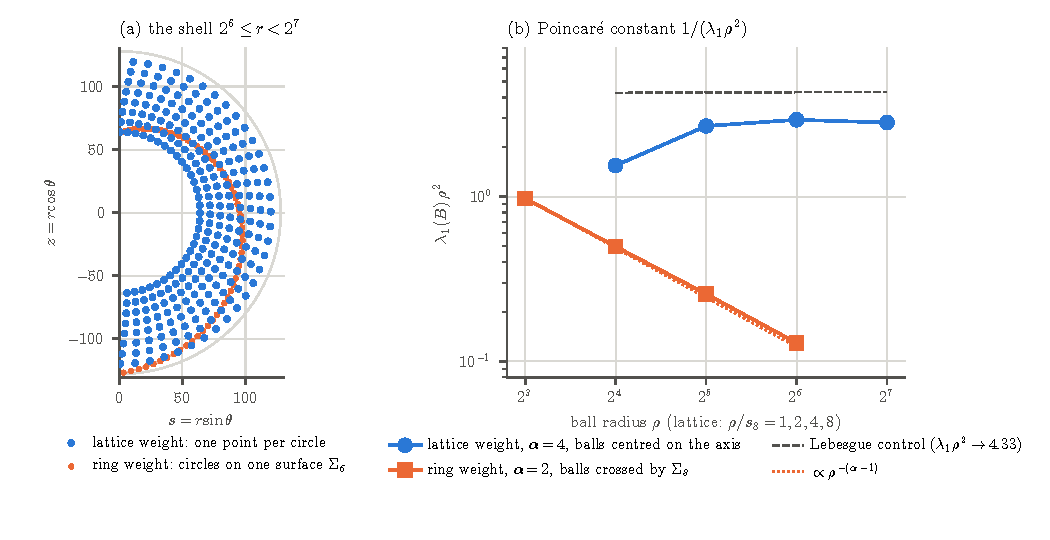
\includegraphics[width=\textwidth]{fig3_lattice_vs_wall.pdf}
\caption{(a) Meridian half-plane of the shell $2^6\le r<2^7$: the circles of
the lattice weight \eqref{eq:w} (one point per circle, spacing $\approx s_6=8$)
and the circles of the ring weight \eqref{eq:wall}, which lie on one surface
$\Sigma_6$ at mesh $\approx3$. (b) $\lambda_1\rho^2$ on balls centred on the
axis: flat for the lattice weight, decaying like $\rho^{-(\alpha-1)}$ for the
ring weight.}
\label{fig:lattice}
\end{figure}

\begin{figure}[t]
\centering
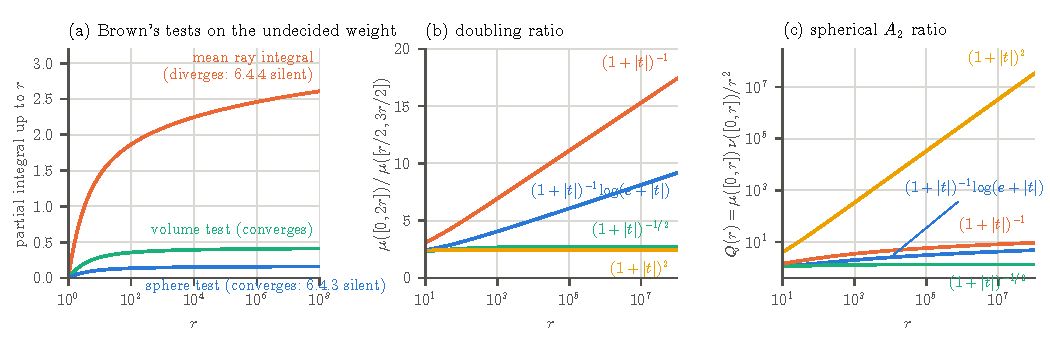
\includegraphics[width=\textwidth]{fig2_undecided.pdf}
\caption{(a) Brown's two tests and the volume test on the product weight of
Proposition~\ref{prop:log}: the sphere integral and the volume integral
converge, the direction-averaged ray integral diverges like $\log\log r$.
(b) The doubling ratio $\mu_1([0,2r])/\mu_1([r/2,3r/2])$ of four
one-dimensional weights $v(t)$. (c) Their spherical $A_2$ ratio on $\R^3$:
bounded only for $(1+\abs t)^{-1/2}$, the one weight that is both doubling and
Poincar\'e (Lemma~\ref{lem:1d}); $(1+\abs t)^2$ is doubling but fails the
Poincar\'e inequality, $(1+\abs t)^{-1}$ is Poincar\'e but not doubling.}
\label{fig:oned}
\end{figure}

\section{Discussion}\label{sec:discussion}

Brown's 1971 theory is the potential theory of the weighted space
$(\R^m,f^*\dd x)$, and his two radial tests are the sphere-area test and a
ray-wise capacity bound. What the later geometric theory adds inside his
undecided zone is now delimited. If the marginal is doubling and Poincar\'e,
nothing is added on the admissible side: parabolicity, Brown's sphere test and
the volume test coincide (Theorem~\ref{thm:A}). On the inadmissible side the
volume test decides weights that no cone of rays decides, and
Theorem~\ref{thm:B} shows that such weights exist in $\R^3$: valleys of
co-dimension two, sweeping every direction at every scale while staying far
apart, are exactly what is needed, and the arithmetic of the construction
($N_k\asymp2^k$ circles, spacing $2^{k/2}$, exponent $\alpha\ge4$) is forced by
the two requirements. Outside the D+P class the zone contains recurrent and
transient members, and the first example of Section~\ref{sec:zone} shows that
the Poincar\'e hypothesis in the volume criterion is not decorative: coherent
circles form a wall, and a wall is recurrent with volume growth $r^3$.

Several questions remain. First, is there a characterization of the undecided
zone without the D+P hypothesis, for instance through the flux test along an
optimally chosen exhaustion, which decided Proposition~\ref{prop:wall}?
Second, the construction of Theorem~\ref{thm:B} is three-dimensional; in the
plane the valleys would be points, transience requires volume growth faster
than $r^2\log r$, and the arithmetic of exponents changes. Third, the relation
between the volume test and the unified sufficient condition of Brown and Hwang
\cite{brownhwang1982} for admissibility should be settled; we expect the lattice
prior not to be covered by a radial condition of any kind, but we have not
checked their hypotheses. Finally, the same parabolic/non-parabolic dichotomy
governs Komaki's shrinkage priors on the Fisher manifold of a model
\cite{komaki2006} (Appendix~\ref{app:komaki}); whether the constructions of
this note have counterparts there is open.

\section*{Acknowledgements}

The question, the choice of what to look for, and the judgement of what
survived are the author's; the labour of making them precise was shared with
large language models used as research assistants, and without them this note
would have taken far longer to write. Claude (Anthropic), run through Claude
Code, read the sources, built and tested the constructions of
Sections~\ref{sec:lattice} and~\ref{sec:zone}, wrote the numerical scripts, and
drafted the text under the author's direction; a second language-model
assistant proposed the cylinder weight of Theorem~\ref{thm:cyl} and the first,
coherent candidate of Section~\ref{sec:wall}, whose failure led to the lattice.
% TODO (owner): name the second assistant (model and provider) if you wish.
Every statement was checked against the cited sources by the author, who is
responsible for the errors that remain. The author thanks The Open University Library for access to the primary
sources. The scripts that produce every number and figure in
Section~\ref{sec:numerics} are available in the public repository
\url{https://github.com/olegroshka/ideg} (directory \texttt{articles/theory}).

\appendix

\section{The same dichotomy for predictive densities}\label{app:komaki}

Brown's criterion is not the only place where parabolicity decides a
statistical question. Let $\{p(x\mid\theta):\theta\in\Theta\subset\R^d\}$ be a
regular parametric model with Fisher metric $g$, Jeffreys prior
$\pi_J\propto\abs g^{1/2}$ and Laplace--Beltrami operator $\Delta_g$
\cite{amari2000}. For a prior $f=e^{-\Phi}\pi_J$, let $\mathrm{Risk}_N(f)$ be
the Kullback--Leibler risk of the Bayesian predictive density built from $N$
observations. Komaki \cite{komaki2006} proved that a prior whose predictive
density asymptotically dominates the Jeffreys one exists if and only if $(M,g)$
carries a Green function, that is, if and only if the Fisher manifold is
non-parabolic (his Theorems~1 and~2; Theorem~3 derives this from negative
sectional curvature for $d\ge3$ through Aomoto's result \cite{aomoto1966}). For
the normal location model the Fisher manifold is flat $\R^d$, the Green
function exists iff $d\ge3$, and the Green prior is Stein's harmonic prior
$\norm\mu^{-(d-2)}$: the predictive analogue of the dichotomy $m\le2$ versus
$m\ge3$ of Table~\ref{tab:dict}.

The quantity that Komaki's expansion produces has a name in geometry. The pair
$(g,\Phi)$ defines the smooth metric measure space $(M,g,e^{-\Phi}\dd V)$,
whose weighted scalar curvature, in Perelman's normalization
\cite[Remark~1.3]{perelman2002}, is
\begin{equation}\label{eq:perelman}
R^{\mathrm m}_\Phi=R+2\Delta_g\Phi-\abs{\nabla\Phi}_g^2 ,
\end{equation}
with $R$ the scalar curvature of $g$; its integral is Perelman's functional
$\mathcal F(g,\Phi)=\int R^{\mathrm m}_\Phi e^{-\Phi}\dd V=\int(R+\abs{\nabla\Phi}^2)e^{-\Phi}\dd V$.

\begin{proposition}\label{prop:komaki}
For a regular model and $f=e^{-\Phi}\pi_J$, with $u=\sqrt{f/\pi_J}=e^{-\Phi/2}$,
\begin{equation}\label{eq:k1}
\mathrm{Risk}_N(\pi_J)-\mathrm{Risk}_N(f)
=\frac{2\Delta_g\Phi-\abs{\nabla\Phi}_g^2}{2N^2}+o(N^{-2})
=\frac{R^{\mathrm m}_\Phi-R}{2N^2}+o(N^{-2})
=-\frac{2}{N^2}\,\frac{\Delta_gu}{u}+o(N^{-2}).
\end{equation}
Hence $f$ asymptotically dominates $\pi_J$ if and only if $u$ is a nonconstant
positive superharmonic function on $(M,g)$, if and only if
$R^{\mathrm m}_\Phi\ge R$ with strict inequality somewhere.
\end{proposition}

\begin{proof}
The first equality is Komaki's expansion \cite[eqs.~(3)--(5)]{komaki2006}: in
the difference of the risks of two priors the prior-independent terms and the
skewness terms cancel. The second is the definition \eqref{eq:perelman}, and
the third is the identity $2\Delta\Phi-\abs{\nabla\Phi}^2=-4\Delta u/u$ for
$u=e^{-\Phi/2}$. The domination statement is Komaki's Theorem~2.
\end{proof}

So the operator that governs domination is $-4\Delta_g$ acting on $u$,
Perelman's operator $-4\Delta+R$ with the potential removed. The scalar
curvature itself has no statistical counterpart:

\begin{proposition}\label{prop:noR}
The prior-independent $O(N^{-2})$ term of the risk of the Jeffreys predictive
density is not proportional to $R$, and $\mathcal F$ is not the integrated risk
reduction: whenever the boundary term of one integration by parts vanishes,
\begin{multline}\label{eq:k2}
\int\bigl(\mathrm{Risk}_N(\pi_J)-\mathrm{Risk}_N(f)\bigr)e^{-\Phi}\dd V
=\frac{1}{2N^2}\int\abs{\nabla\Phi}^2_ge^{-\Phi}\dd V+o(N^{-2})\\
=\frac{1}{2N^2}\Bigl[\mathcal F(g,\Phi)-\int R\,e^{-\Phi}\dd V\Bigr]+o(N^{-2}).
\end{multline}
\end{proposition}

\begin{proof}
Komaki \cite[Theorem~A1, eq.~(29)]{komaki2015} gives the full $O(N^{-2})$ risk
of the Jeffreys predictive density. Its prior-independent part is a fixed
combination of the exponential and mixture embedding curvatures, the squared
norm of the skewness tensor, a fourth-moment contraction and one mixed moment.
For $d=1$ these are generically nonzero, Efron's statistical curvature of a
curved exponential family being the simplest instance \cite{efron1975}, while
every intrinsic curvature of a one-dimensional Riemannian manifold vanishes.
Equation \eqref{eq:k2} follows from \eqref{eq:k1} and
$\int\Delta_g\Phi\,e^{-\Phi}\dd V=\int\abs{\nabla\Phi}^2e^{-\Phi}\dd V$.
\end{proof}

Two remarks complete the parallel. First, Komaki's treatment of vague priors
\cite[\S3]{komaki2006} decides domination over $h=e^{-\Phi}\pi_J$, $d\ge3$, by
superharmonicity with respect to the conformal metric
$\tilde g=(h/\pi_J)^{2/(d-2)}g$: changing the reference prior is a conformal
change of the Fisher metric, and for Stein's prior on $\R^d$ the conformal
metric is the flat cylinder $S^{d-1}\times\R$ with the origin pushed to
infinite distance (his Example~1). Second, in both theories the geometry of the
prior enters through recurrence or transience of a diffusion, Brown's on the
sample space and Komaki's on the parameter space, and not through curvature in
a risk formula. Whether the scattered valleys of Theorem~\ref{thm:B}, which
separate the volume test from the sphere test on $\R^3$, have an analogue on a
Fisher manifold, where Komaki's criterion would then separate the existence of a
shrinkage prior from the sphere-area growth of the model, is open.

\bibliographystyle{amsplain}
{\small
\bibliography{references}
}

\end{document}
